\documentclass[tikz,border=10pt]{standalone}
\usepackage{tikz}
\usetikzlibrary{shapes.geometric, arrows.meta, positioning, fit, backgrounds}

\tikzset{
    box/.style={rectangle, rounded corners, minimum width=3.5cm, minimum height=2.1cm, text centered, draw=black, thick, font=\normalsize},
    process/.style={box, fill=blue!15},
    data/.style={box, fill=green!15},
    module/.style={box, fill=orange!15},
    decision/.style={box, fill=purple!15},
    arrow/.style={thick,-{Stealth[length=2mm]}},
    dashedarrow/.style={thick,-{Stealth[length=2mm]},dashed}
}

\begin{document}
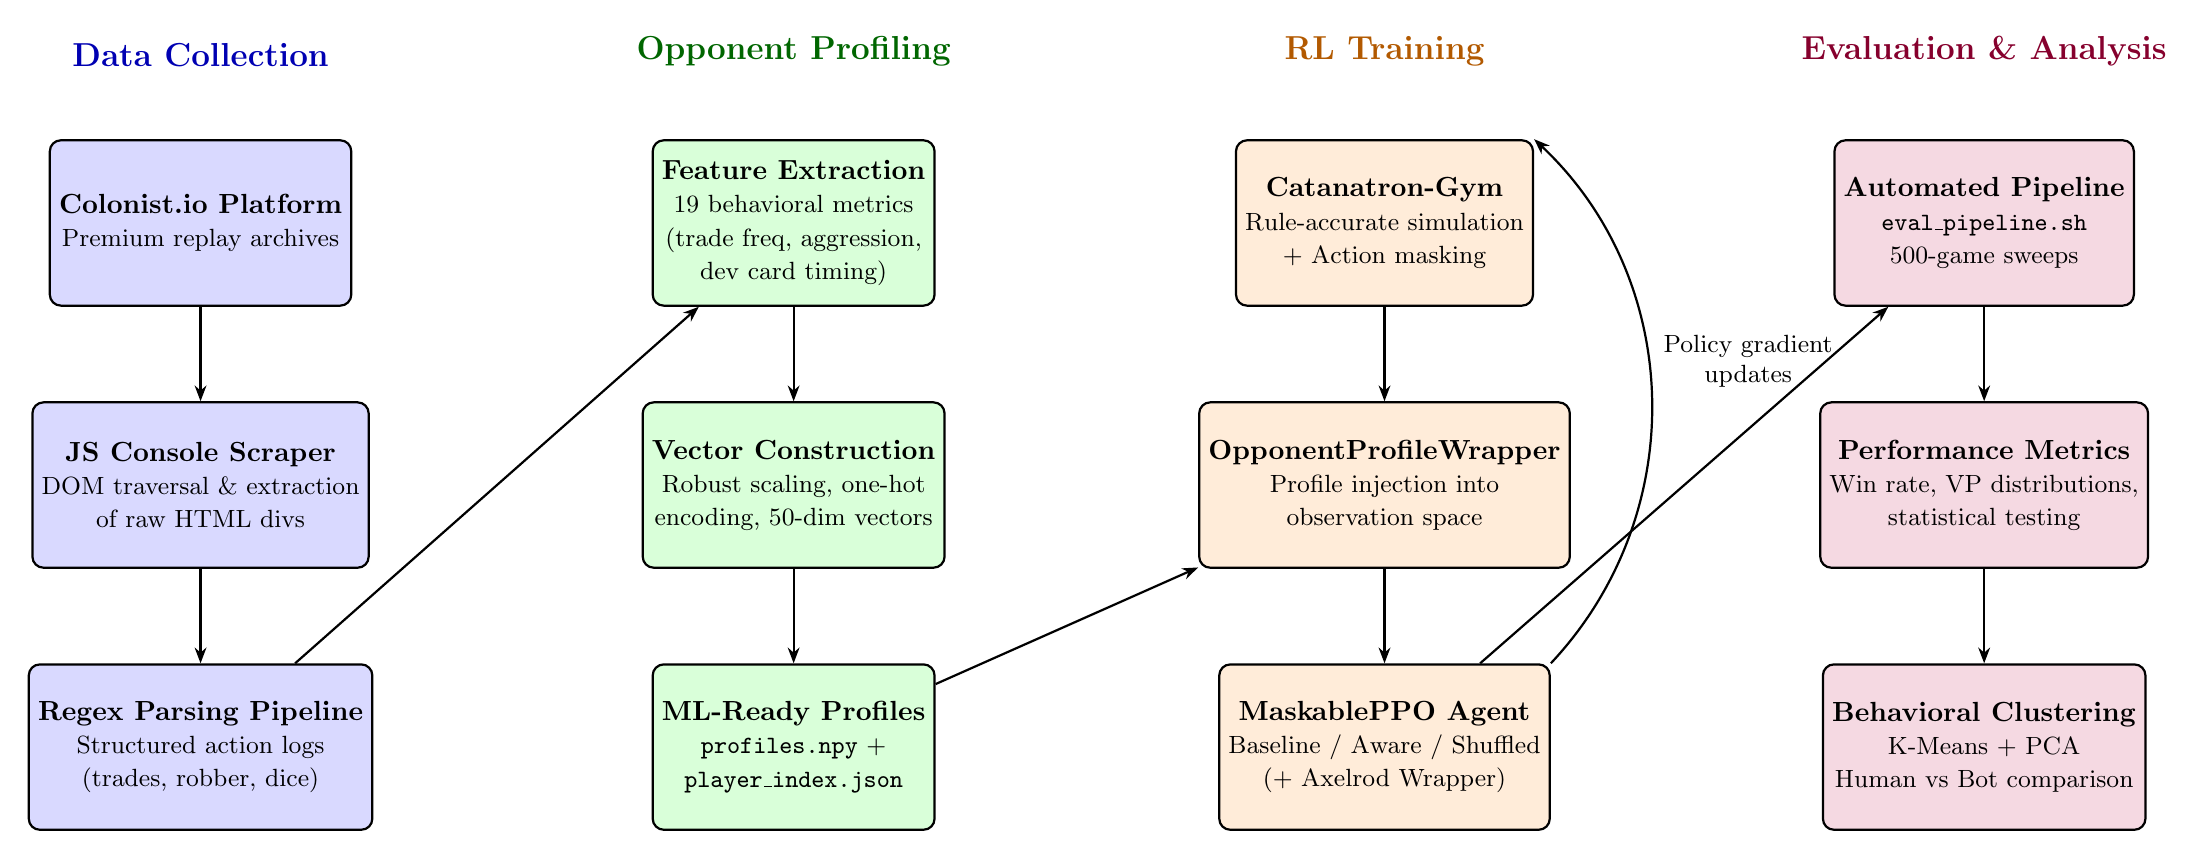
\begin{tikzpicture}[node distance=1.2cm and 3.8cm, every text node part/.style={align=center}]

% Layer 1: Data Collection
\node (colonist) [process] {\textbf{Colonist.io Platform}\\\small Premium replay archives};
\node (scraper) [process, below=of colonist] {\textbf{JS Console Scraper}\\\small DOM traversal \& extraction\\\small of raw HTML divs};
\node (parser) [process, below=of scraper] {\textbf{Regex Parsing Pipeline}\\\small Structured action logs\\\small (trades, robber, dice)};

% Layer 2: Opponent Profiling
\node (extract) [data, right=of colonist] {\textbf{Feature Extraction}\\\small 19 behavioral metrics\\\small (trade freq, aggression,\\\small dev card timing)};
\node (scale) [data, below=of extract] {\textbf{Vector Construction}\\\small Robust scaling, one-hot\\\small encoding, 50-dim vectors};
\node (profiles) [data, below=of scale] {\textbf{ML-Ready Profiles}\\\small \texttt{profiles.npy} +\\\small \texttt{player\_index.json}};

% Layer 3: RL Training
\node (gym) [module, right=of extract] {\textbf{Catanatron-Gym}\\\small Rule-accurate simulation\\\small + Action masking};
\node (wrapper) [module, below=of gym] {\textbf{OpponentProfileWrapper}\\\small Profile injection into\\\small observation space};
\node (ppo) [module, below=of wrapper] {\textbf{MaskablePPO Agent}\\\small Baseline / Aware / Shuffled\\\small (+ Axelrod Wrapper)};

% Layer 4: Evaluation & Analysis
\node (pipeline) [decision, right=of gym] {\textbf{Automated Pipeline}\\\small \texttt{eval\_pipeline.sh}\\\small 500-game sweeps};
\node (metrics) [decision, below=of pipeline] {\textbf{Performance Metrics}\\\small Win rate, VP distributions,\\\small statistical testing};
\node (cluster) [decision, below=of metrics] {\textbf{Behavioral Clustering}\\\small K-Means + PCA\\\small Human vs Bot comparison};

% Horizontal data flow
\draw [arrow] (parser) -- (extract);
\draw [arrow] (profiles) -- (wrapper);
\draw [arrow] (ppo) -- (pipeline);

% Vertical processing flow
\draw [arrow] (colonist) -- (scraper);
\draw [arrow] (scraper) -- (parser);
\draw [arrow] (extract) -- (scale);
\draw [arrow] (scale) -- (profiles);
\draw [arrow] (gym) -- (wrapper);
\draw [arrow] (wrapper) -- (ppo);
\draw [arrow] (pipeline) -- (metrics);
\draw [arrow] (metrics) -- (cluster);

% Training feedback loop
\draw [arrow, bend right=45] (ppo.north east) to node[above right, font=\small, text width=2.2cm] {Policy gradient updates} (gym.north east);

% Layer labels
\node[above=0.8cm of colonist, font=\large\bfseries, blue!70!black] {Data Collection};
\node[above=0.8cm of extract, font=\large\bfseries, green!40!black] {Opponent Profiling};
\node[above=0.8cm of gym, font=\large\bfseries, orange!70!black] {RL Training};
\node[above=0.8cm of pipeline, font=\large\bfseries, purple!70!black] {Evaluation \& Analysis};

\end{tikzpicture}
\end{document}
